\documentclass{article}
\usepackage[utf8]{inputenc}
\usepackage{graphicx}
\usepackage{amsmath}

\title{Inverted Pendulum with inertial Wheel }
\author{Amato Pierluigi}
\date{November 2018}

\begin{document}

\maketitle

\section{Dinamica}
Il sistema in figura \ref{fig:InvertedPendulum} è studiato in maniera monodimensionale.

\begin{figure}[htp]
\centering
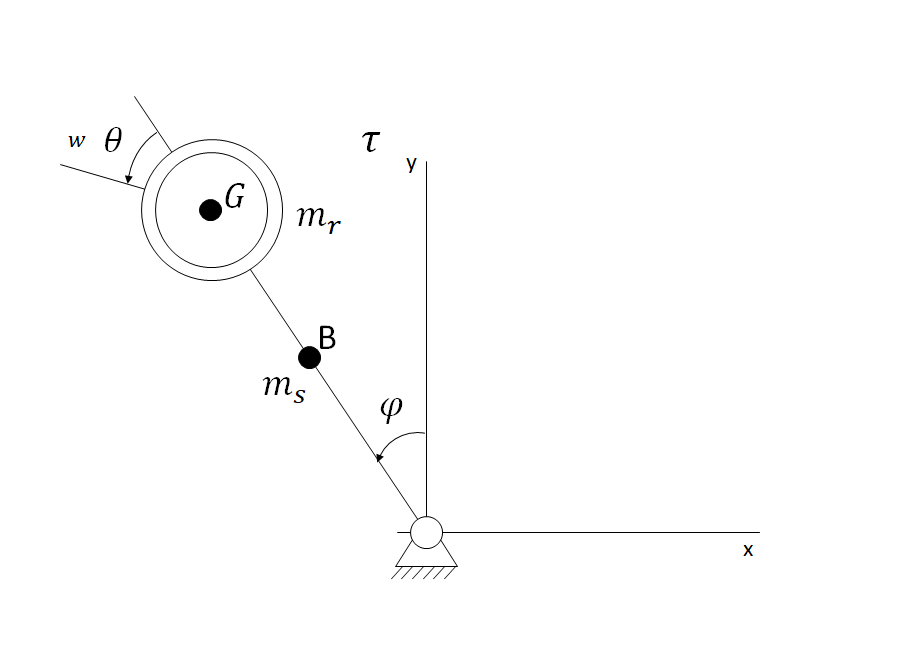
\includegraphics[width=10cm]{img/Pendolo.png}
\caption{Inverted Pendulum with Inertial Wheel}
\label{fig:InvertedPendulum}
\end{figure}

L'obiettivo è quello di utilizzare la formulazione di Lagrange per ottenere la dinamica, linearizzare e poi fare le simulazioni per riuscire a valutare la coppia che il motore deve riuscire a garantire.
Le equazioni della energia cinetica e dell'energia potenziale sono le seguenti:

\begin{gather}
T = \frac{1}{2}m_sv_B^2+\frac{1}{2}m_rv_G^2+\frac{1}{2}I_B\dot{\psi}^2+\frac{1}{2}I_G(\dot{\psi}+\dot{\theta})^2 \\
U = m_sg\frac{L}{2}cos(\psi)+m_rgLcos(\psi)
\end{gather}

dove L è l'asta del pendolo, $m_r$ la massa del rotore, $m_s$ la massa dell'asta, i punti B e G sono i due baricentri dell'asta e del rotore.
L'inerzia  $I_B$ e $I_G$ sono le inerzie della massa del pendolo e della ruota.

\begin{align*}
&OB = \frac{L}{2}(sin(\psi)\hat{i}+cos(\psi)\hat{j})\notag\\
&OG = L(sen\psi\hat{i}+cos(\psi)\hat{j})\notag\\
&v_B = L\dot{\psi}(-cos(\psi)\hat{i}+sen(\psi)\hat{j})\notag\\
&v_G = L\dot{\psi}(-cos(\psi)\hat{i}+sen(\psi)\hat{j})\notag\\
&I_G = Solidworks\\
&I_B = Solidworks
\end{align*}

Avendo espresso le velocità in questo modo la T diventa in questo modo:
\begin{gather}
T = \frac{1}{2}(m_s\frac{L^2}{4})\dot{\psi}^2+
\frac{1}{2}(m_rL^2)\dot{\psi}^2+
\frac{1}{2}I_B\dot{\psi}^2+
\frac{1}{2}I_G(\dot\psi^2+\dot{\theta}^2+2\dot\psi\dot\theta)
\end{gather}
\begin{gather}
T = \frac{1}{2}[m_s(\frac{L}{2})^2+m_r(L)^2+I_B+I_G]\dot{\psi}^2+
\frac{1}{2}I_G\dot{\theta}^2+I_G\dot\psi\dot\theta\\
U = [m_s(\frac{L}{2})^2+m_r(L)^2]cos(\psi)
\end{gather}
raccolgo i termini:
\begin{align}
&I_{T} = m_s(\frac{L}{2})^2+m_r(L)^2+I_B+I_G\\
&G_1 = m_s(\frac{L}{2})^2+m_r(L)^2
\end{align}

\begin{align}
L &= T-U\\
L &= \frac{1}{2}I_{T}\dot{\psi}^2+\frac{1}{2}I_G\dot{\theta}^2+I_G\dot\psi\dot\theta-G_1cos(\psi)
\end{align}
Calcolo la derivata rispetto alle variabili $\dot\theta$ e  $\dot\psi$ ottenendo:
\begin{align}
&\frac{dL}{d\dot\psi} = I_{T}\dot{\psi} + I_G\dot\theta\\ 
&\frac{dL}{d\dot\theta} = I_G\dot{\psi} + I_G\dot{\theta}\\
&\frac{d}{dt}\frac{dL}{d\dot\psi} = I_{T}\ddot{\psi} + I_G\ddot\theta\\
&\frac{d}{dt}\frac{dL}{d\dot\theta} =  I_G\ddot\psi + I_G\ddot\theta
\end{align}
mentre la derivata rispetto alle variabili non derivate:
\begin{align}
\frac{dL}{d\psi} & = G_1 sin(\psi)\\
\frac{dL}{d\theta} & = 0
\end{align}
Applicando i vari termini ottenuti fin'ora nella equazione di Lagrange:
\begin{align*}
&\frac{d}{dt}\frac{dL}{d\dot q}-\frac{dL}{dq} = Q_nc
\end{align*}

Ottenendo quindi due equazioni della forma:
\begin{align}
&
\begin{cases}
I_T\ddot{\psi} + I_G\ddot\theta - G1sin(\psi) = 0\\
I_G\ddot\psi + I_G\ddot\theta = \tau
\end{cases}
\end{align}
dove ho imposto $G1 = m_sg\frac{L}{2}+m_rgL$.
Scrivo tutto in forma matriciale ottenendo:
\[ B =
\begin{bmatrix}
I_T & I_G\\
I_G & I_G
\end{bmatrix}
\quad
G = 
\begin{bmatrix}
-G1sin(\psi)\\
0
\end{bmatrix}
\]
quindi l'equazione della dinamica del nostro sistema:
\begin{equation}
\begin{bmatrix}
I_T & I_G\\
I_G & I_G
\end{bmatrix}
\begin{bmatrix}
\ddot\psi\\
\ddot\theta
\end{bmatrix}
+
\begin{bmatrix}
-G1sin(\psi)\\
0
\end{bmatrix}
=
\begin{bmatrix}
0\\
\tau
\end{bmatrix}
\end{equation}
\subsection{Spazio degli stati}
Il sistema di due equazioni differenziali viene disaccoppiato nell'ipotesi in cui ci sia la possibilità di controllarlo escludendo la dinamica del motore. Verrà poi analizzata la coppia da generare usando la seconda equazione.
Impongo un vettore dello spazio degli stati in questo modo:
\begin{align*}
&x = [\psi,\dot\psi,\dot\theta]^T \notag =[x_1,x_2,x_3]^T \notag\\ 
&u = \tau
\end{align*}
Il sistema non linearizzato diviene:
\[
\begin{cases}
I_T\dot{x_2}+I_G\dot{x_3} = G1sin(x_1)\\
I_G\dot{x_2}+I_G\dot{x_3} = u\\
\end{cases}
\]
Utilizzando Cramer:
\begin{gather}
\Delta = I_T I_G - I_G I_G\\
\dot{x_2} = \frac{\begin{bmatrix}
G1sin(x_1) & I_G\\
u & I_G
\end{bmatrix}}
{\Delta}\\
\dot{x_3} = \frac{\begin{bmatrix}
I_T &  G1sin(x_1)\\
I_G &  u
\end{bmatrix}}
{\Delta}
\end{gather}
\begin{align*}
&\dot{x_1} = x_2\\
&\dot{x_2} = \frac{G1sin(x_1)I_G}{\Delta} -\frac{I_G}{\Delta}u\\
&\dot{x_3} = -\frac{G1sin(x_1)I_G}{\Delta} +\frac{I_T}{\Delta}u\\
\end{align*}
Che linearizzato attorno a $\psi = 0$
\begin{align*}
\begin{bmatrix}
\dot{x_1}\\
\dot{x_2}\\
\dot{x_3}\\
\end{bmatrix}
=
\begin{bmatrix}
0&1&0\\
\frac{G_1 I_G}{\Delta}&0&0\\
-\frac{G_1 I_G}{\Delta}&0&0
\end{bmatrix}
\begin{bmatrix}
x_1\\
x_2\\
x_3\\
\end{bmatrix}
+
\begin{bmatrix}
0\\
-\frac{I_G}{\Delta}\\
\frac{I_T}{\Delta}\\
\end{bmatrix}
u
% &\dot{x_1} = x_2\\
% &\dot{x_2} = -\frac{G1sin(x_1)I_G}{\Delta} -\frac{I_G}{\Delta}u\\
% &\dot{x_3} = \frac{G1sin(x_1)I_G}{\Delta} -\frac{I_T}{\Delta}u\\
\end{align*}
Una volta ricavate le inerzie tramite il tool di design, ricordando che il calcolo viene eseguito in caso monodimensionale, viene applicato un controllo PD con simulink


\end{document}

